\documentclass{article}
\usepackage[a4paper, total={6in, 8in}]{geometry}
\usepackage[utf8]{inputenc}
\frenchspacing

% ------------------------------------------------------------
\usepackage{caption}
\captionsetup{labelformat=empty,labelsep=none}
\usepackage{scalerel,stackengine,amsmath}
\usepackage{mathtools}
\usepackage{dsfont}
\usepackage{multicol}
\usepackage{algorithm2e}
\usepackage{amsfonts}
\usepackage{enumerate}
\usepackage{enumitem}
% ------------------------------------------------------------

% image
\newcommand{\incl}[2]{\includegraphics[width=#1\textwidth]{#2}}
\newcommand{\inclc}[2]{\begin{center}\includegraphics[width=#1\textwidth]{#2}\end{center}}
% description
\newcommand{\thetitle}{}
\newcommand{\thecontents}{}
\newcommand{\thedate}{}
\newcommand{\theauthor}{}
\newcommand{\thedescription}{
	\section*{\thetitle}
	\begin{tabular}{ll}%
	Inhalt:&\thecontents\\%
	Datum:&\thedate\\%
	Author:&\theauthor\\%
	\end{tabular}%
}
% -- math mode stuff
\newcommand{\meq}[1]{\begin{equation*}\begin{aligned}#1\end{aligned}\end{equation*}}
% \newcommand{\NN}{\mathbb{N}}
\newcommand{\NN}{\mathbb{N}}
\newcommand{\ZZ}{\mathbb{Z}}
\newcommand{\QQ}{\mathbb{Q}}
\newcommand{\RR}{\mathbb{R}}
\newcommand{\CC}{\mathbb{C}}
\newcommand{\subt}[1]{\normalfont{(#1)}}
\newcommand{\ifcases}[2]{\begin{equation*}#1\begin{cases}#2\end{cases}\end{equation*}}
\newcommand{\ring}[1]{(#1,+,\cdot)}
\newcommand{\estimates}{\mathrel{\hat{=}}}
\newcommand{\OO}{\mathcal{O}}
\newcommand{\LRA}{\Leftrightarrow}
\newcommand{\LA}{\Leftarrow}
\newcommand{\RA}{\Rightarrow}
\newcommand{\textabove}[2]{\mathrel{\stackrel{\makebox[0pt]{\mbox{\normalfont\tiny #1}}}{#2}}}
\newcommand{\myqed}[1]{\hfill$\Box${\footnotesize#1}}
\newcommand{\neo}[1]{\begin{pmatrix}#1\end{pmatrix}}
\newcommand{\SsS}{\mathcal{S}}
\newcommand{\correct}{\hfill\checkmark}
\newcommand{\ubr}[2]{\underbrace{#1}_{\mathclap{\text{#2}}}}
\newcommand{\obr}[2]{\overbrace{#1}^{\mathclap{\text{#2}}}}
\renewcommand{\star}{^*}
\newcommand{\blank}{\ttt{\textvisiblespace}}
\newcommand\equalhat{\mathrel{\stackon[1.5pt]{=}{\stretchto{%
    \scalerel*[\widthof{=}]{\wedge}{\rule{1ex}{3ex}}}{0.5ex}}}}
\newcommand{\correspondsto}{\equalhat}
\newcommand{\weg}{(weggelassen)}
\newcommand{\chf}{\mathds{1}}
	% -- enumerations
\newcommand{\abc}[1]{\begin{enumerate}[label=\alph*.]#1\end{enumerate}}
\newcommand{\num}[1]{\begin{enumerate}[label=\arabic*.]#1\end{enumerate}}
\newcommand{\bul}[1]{\begin{itemize}#1\end{itemize}}
% -- text mode stuff
% \newcommand{\note}[1]{(\textit{#1})}
\newcommand{\ttt}{\texttt}
\newcommand{\tbf}{\textbf}
\newcommand{\tit}{\textit}
\newcommand{\trt}{\textit}
\newcommand{\tsc}{\textsc}
\newcommand{\tul}{\underline}
\newcommand{\tsub}[1]{\tre{\large#1}}
% -- text input stuff
\newcommand{\ditto}{''}
% <warning_emoji>
\newcommand*{\TakeFourierOrnament}[1]{{%
\fontencoding{U}\fontfamily{futs}\selectfont\char#1}}
\newcommand*{\warning}{\TakeFourierOrnament{66}}
\newcommand{\warn}{{\Large\warning}\ \ }
% </warning_emoji>
% logic stuff
\newcommand{\tttrue}{\ttt{true}}
\newcommand{\fffalse}{\ttt{false}}
% algorithm stuff:
\newcommand{\wwhile}{\textbf{while}}
\newcommand{\ffor}{\textbf{for}}
\newcommand{\ggoto}{\textbf{goto}}
\newcommand{\ddo}{\textbf{do}}
\newcommand{\iif}{\textbf{if}}
\newcommand{\tthen}{\textbf{then}}
\newcommand{\eelse}{\textbf{else}}
\newcommand{\eend}{\textbf{end}}
\newcommand{\hhalt}{\textbf{halt}}
\newcommand{\aand}{\textbf{and}}
\newcommand{\oor}{\textbf{or}}
\newcommand{\ffunction}{\textbf{function}}
\newcommand{\rreturn}{\textbf{return}}
\newcommand{\cccc}{\hphantom{cccc}}
\newcommand{\ccc}{\hphantom{ccc}}
\newcommand{\cc}{\hphantom{cc}}
\renewcommand{\;}{;\\}
\newcommand{\cmt}[1]{\ttt{#1}}
\newcommand{\lims}{\limsup_{n\to\infty}}
\newcommand{\limi}{\liminf_{n\to\infty}}
\newcommand{\true}{\ttt{true}}
\newcommand{\false}{\ttt{false}}


% <local>
\usepackage{hyperref}
\usepackage{tikz}
\usepackage{titlesec}
% --------
\newcommand{\pickl}[1]{\begin{center}\hrulefill\ \texttt{[ \textbf{Pickl #1} ]}\ \hrulefill\end{center}}
\newcommand{\PP}{\mathbb{P}}
\newcommand{\Pcal}{\mathcal{P}}
\renewcommand{\thesection}{\Roman{section}}
\setcounter{tocdepth}{2}
\renewcommand{\contentsname}{Inhaltsverzeichnis}
% </local>

\renewcommand{\thetitle}{Stochastik}
\renewcommand{\thecontents}{Live-Transkription}
\renewcommand{\thedate}{SS 2024}
\renewcommand{\theauthor}{Prof. Dr. Peter Pickl}

\begin{document}
\thedescription
\tableofcontents
\newpage

\pickl{15.04.2024}
\trt{In der Stochastik geht es um die Modellierung von Experimenten, deren Ausgang vom Zufall abh\"angt.}
\section{Endliche Wahrscheinlichkeitsr\"aume}
\subsection{Ergebnismenge, Ereignismenge}
\subsubsection{Definition (Ergebnismenge)}
Die Menge $\Omega$, welche die m\"oglichen Ausg\"ange eines Zufallexperiementes beschreibt, dennen wir \trt{Grundmenge} oder \trt{Ergebnismenge}.
\subsubsection{Definition (Ereignismenge)}
Die Potenzmenge $\mathcal{P}(\Omega)$, d.h. die Menge aller Teilmengen $\Omega$, nennen wir \trt{Ereignismenge}.
\subsubsection{Beispiel}
\num{
\item Wir werfen einen W\"urfel.
\bul{
\item $\Omega=\{1,2,\ldots,6\}$,
\item $\mathcal{P}(\Omega)=\{\emptyset,\Omega,\{1\},\ldots,\{1,1\},\ldots\}$,
}
\item Gl\"ucksrad: $\Omega=[0,2\pi[$ beschreibt die m\"oglichen Winkel eines Gl\"uckradspiels. $\mathcal{P}(\Omega)$ ist klar (keine geeignete Ereignismenge, siehe Kapitel 2).
}
\subsection{Wahrscheinlichkeitsma\ss{}}
Das Wahrscheinlichkeitsma\ss{} wird auf der Ereignismenge definiert. Grund: F\"ur \"uberabz\"ahlbare Mengen (Gl\"ucksrad z.B.) haben einzelne Ausg\"ange h\"aufig Wahrscheinlichkeit $0$, obwohl global gesehen existiert ein sinnvolles Wahrscheinlichkeitsma\ss{} (siehe Kapitel 2).
\\~\\
Die Wahrscheinlichkeit quantifiziert die Plausibilit\"at der entsprechenden Ereignisse. Sie gibt die relative H\"aufigkeit an, wie oft ein bestimmtes Ereignis nach sehr h\"aufigen Wiederholen unter identischen Umst\"anden eintritt.
\subsubsection{Definition (Wahrscheinlichkeitsma\ss{})}
Eine Abbildung $\PP\colon\mathcal{P}(\Omega)\to\RR$ nennt man \trt{Wahrscheinlichkeitsma\ss{}} $:\LRA$
\abc{
\item[\tbf{K}a)] $\PP(A)\geq0,\ \forall A\subset\Omega$,
\item[\tbf{K}b)]  $\PP(\Omega)=1$,
\item[\tbf{K}c)]  $\PP(A\cup B)=\PP(A)+\PP(B),\ \forall A,B\subset\Omega,\ A\cap B=\emptyset$.
}
\subsubsection{Bemerkung}
Die Axiome a)-c) nennt man \trt{Axiome von Kolmogorov} (werden in 2 ebenfalls leicht angepasst).
\subsubsection{Satz}
F\"ur jedes Wahrscheinlichkeitsma\ss{} $\PP\colon\mathcal{P}(\Omega)\to\RR$ f\"ur beliebiges $\Omega$ gelten:
\abc{
\item $\PP(A^C)=1-\PP(A),\ \forall A\subset\Omega$.
\item $\PP(A)\leq1$.
\item $\PP(A\cup B)=\PP(A)+\PP(B)-\PP(A\cap B)$.
}
\subsubsection{Beweis}
\weg
\subsubsection{Bemerkung}
\"Uber die Wahrscheinlichkeiten der Elementarereignisse (d.h. der einelementigen Ereignisse), wird das Wahrscheinlichkeitsma\ss{} eindeutig festgelegt.
\\~\\
Betrachte $\PP(A)$ f\"ur $A=\{w_1,w_2,\ldots,w_k\}\subset\Omega$. Durch mehrmaliges Anwenden von \tbf{K}c) erh\"alt man
\meq{\PP(A)=\sum_{i=1}^{k}\PP(\{w_k\}).}
\subsubsection{Definition (Wahrscheinlichkeitsraum)}
Das Paar $(\Omega,\PP)$ nennt man auch \trt{Wahrscheinlichkeitsraum} (auch $(\Omega,\mathcal{P}(\Omega),\PP)$).


\pickl{18.04.2024}
\subsubsection{Bemerkung}
Wie findet man nun das richtige Wahrscheinlichkeitsma\ss{}, d.h. jenes, welches zu meinem Experiment passt?
\num{
\item Ausprobieren (siehe unten, ``Statistik'').
\item Analyse der physikalischen Eigenschaften. Praktikabel, falls Symmetrie in den relevanten physikalischen Eigenschaften herrscht:
}
\subsubsection{Laplace-Annahme (Indifferenzprinzip)}
Falls es keinen Grund zur Annahme gibt, dass die verschiedenen Ausg\"ange des Experiments im Wesentlichen zu unterscheiden sind, nehmen wir an, dass die Wahrscheinlichkeiten aller Elementarerignisse gleich sind.
\subsubsection{Folgerung}
Sei $\Omega$ ein Ergebnisraum. Unter der Laplace-Annahme gilt:
\[
\mathbb{P}(A)=\frac{|A|}{|\Omega|}
\]
\subsubsection{Beweis}
\[
1\textabove{\tbf{K}}{=}\mathbb{P}(\Omega)=\mathbb{P}(\bigcup_{\omega\in\Omega}\{\omega\})\textabove{\tbf{K}}{=}\sum_{\omega\in\Omega}\mathbb{P}(\{\omega\})\textabove{\tbf{L}}{=}|\Omega|\cdot\mathbb{P}(\{\omega\})
\]
$\Rightarrow\forall\omega\in\Omega$ gilt:
\[
\mathbb{P}(\{w\})=\frac{1}{|\Omega|}.
\]
Au\ss{}erdem:
\[
\mathbb{P}(A)=\mathbb{P}(\bigcup_{\omega\in A}\{\omega\})\textabove{\tbf{K}}{=}\sum_{\omega\in A}\mathbb{P}(\{\omega\})=|A|\cdot\frac{1}{|\Omega|}.
\]
\subsubsection{Beispiel}
\num{
\item Werfen eines ungezinkten W\"urfels:
\[
\mathbb{P}(\{2,4,6\})=\frac{3}{6}=\frac{1}{2}.
\]
\item Gesamte Augenzahl bei zweimaligen Werfen des W\"urfels
\[
\Omega=\{2,\ldots,12\},
\]
Laplace-Annahme gilt nicht. Die Elemente sind wesentlich verschieden, z.B. $2$ hat nur Option $(1,1)$, $7$ hat die Optionen $\{(1,6),\ldots\}$.
\item Ziegenproblem: Wir befinden uns in einer Gameshow, d\"urfen zwischen drei Toren w\"ahlen. Hinter einemal Tor ist ein Gewinn, hinter zweien eine Niete. Der Moderator \"offnet eines der nicht-gew\"ahlten Tore. Hinter diesen ist eine Niete. Er bietet daraufhin an, das Tor zu wechseln. Ist der Wechsel sinnvoll?
\bul{
\item Problem 1: Spielregeln m\"ussen erg\"anzt werden. Wie handelt der Moderator? Wir gehen davon aus, dass er oder sie in jedem Fall ein nicht-gew\"ahltes Tor mit Niete \"offnet.
\item Problem 2: Man ist geneigt, von einer Laplace-Situation auszugehen. Dies ist falsch, da die Tore durch die Wahl und die Reaktion des Moderators zu unterscheiden sind.
}
}
\begin{center}
\begin{minipage}{0.45\textwidth}
\centering
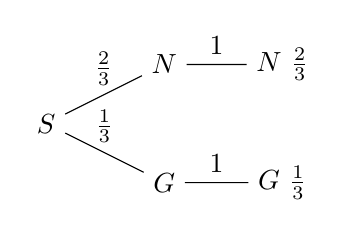
\begin{tikzpicture}[grow=right]
    \node {$S$}
        child
        {
            node {$G$}
            child
            {
                node {$G\ \frac{1}{3}$}
                edge from parent node[above] {$1$}
            }
            edge from parent node[above] {$\frac{1}{3}$}
        }
        child
        {
            node {$N$}
            child
            {
                node {$N\ \frac{2}{3}$}
                edge from parent node[above] {$1$}
            }
            edge from parent node[above] {$\frac{2}{3}$}
        };
\end{tikzpicture}\\
Ohne Wechseln
\end{minipage}
\begin{minipage}{0.45\textwidth}
\centering
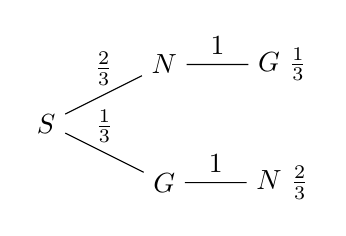
\begin{tikzpicture}[grow=right]
    \node {$S$}
        child
        {
            node {$G$}
            child
            {
                node {$N\ \frac{2}{3}$}
                edge from parent node[above] {$1$}
            }
            edge from parent node[above] {$\frac{1}{3}$}
        }
        child
        {
            node {$N$}
            child
            {
                node {$G\ \frac{1}{3}$}
                edge from parent node[above] {$1$}
            }
            edge from parent node[above] {$\frac{2}{3}$}
        };
\end{tikzpicture}\\
Mit Wechseln
\end{minipage}
\end{center}
mit Start ($S$), Gewinn ($G$) und Niete ($N$).
\subsection{Kombinatorik}
Wie bestimmt man in einer Laplace-Situation $|A|$ und $|\Omega|$?
\subsubsection{Beispiele}
\abc{
\item Sei $\Omega=A\times B$, so ist $|\Omega|=|A|\cdot|B|$ M\"unzwurf, dann W\"urfel:
\[
A=\{\text{K},\text{Z}\},\ B=\{1,\ldots,6\}.
\]
\item Urne mit $N$ durchnummerierten Kugeln. Wir ziehen davon nacheinander ohne Zur\"ucklegen $k$ Kugeln (Reihenfolge wird ber\"ucksichtigt):
\[
|\Omega|=N(N-1)\ldots(N-k+1)=\frac{N!}{(N-k)!}.
\]
\item Zahlenlotto ``6 aus 49'', wie b) ohne R\"ucksicht auf Reihenfolge:
\[
|\Omega|=\frac{N!}{(N-k)!}\cdot\frac{1}{k!}.
\]
\item Anzahl der Anagramme von \ttt{MISSISSIPPI}.
\[
|\Omega|=\frac{11!}{\ubr{4!}{\ttt{I}}\ubr{4!}{\ttt{S}}\ubr{2!}{\ttt{P}}}.
\]
}
\newpage
\section{Allgemeine Wahrscheinlichkeitsr\"aume}
\setcounter{subsection}{-1}
\subsection{Anpassung des 3. Axioms von Kolmogorov}
Wir werden das 3. Axiom von Kolmogorov anpassen:
\[
\mathbb{P}(\bigcup_{j=1}^\infty A_j)=\sum_{j=1}^\infty\mathbb{P}(A_j),\ \text{falls}\ A_j\cap A_k=\emptyset,\ \forall j\neq k.
\]
Schwieriger ist die anpassung des Definitionsbereiches von $\mathbb{P}$. Warum ist das n\"otig? Betrachte das Beispiel ``Gl\"ucksrad''. 


\end{document}

